\documentclass[__minimum__.tex]{subfiles}

\begin{document}
	\begin{definition}
	Выражение $\hat{H}\psi = E\psi$ называется стационарным уравнением Шредингера, где $E = \hbar \omega$ - соотношение Эйнштейна.\\
	\end{definition}
	\begin{definition}
	Симметричная волновая функция описывает частицы, называемые бозонами.\\
	Бозоны - частицы с целым спином $(s = 0,1,2...)$\\
	Антисимметричная волновая функция описывает частицы, называемые фермионами.\\
	Фермионы - частицы с полуцелым спином $(s = \frac{1}{2},\frac{3}{2},\frac{5}{2}...)$\\
	\end{definition}
	\textbf{Эрмитов оператор}\\
	$\hat{A}\left|j\right> = a_j\left|j\right>$\\
	\textbf{Принцип неразичимости частиц одного сорта}\\
	В классической механике всегда есть возможность различить (пронумеровать объекты и сохранить нумерацию в течении всего времени их существования) одинаковые объекты, в то время как квантовомеханическое описание делает невозможным различить одинаковые объекты.
	\begin{gather}
	<x|\hat{A}|x> = <\widetilde{x}|\hat{A}|\widetilde{x}>
	\end{gather}
	- это математическая формулировка принципа неразличимости частиц. Не существует наблюдаемых отличий между системой в состоянии $|x>$ и состемой в состоянии $|\widetilde{x}> = \hat{P}|x>$, где $\hat{P}$ - \textit{оператор перестановки}
	\begin{definition}
	$\hat{P}$ -оператор перестановки, в основе его определения лежит действие на базисные векторы $|i> |j>$. Это означает, что под действием оператора на 2-хчастичное состояние, в котором 1-я частица находилась в состоянии $|i>$, а 2-я в состоянии $|j>$, получается 2-хчастичное состояние, в котором 1-я частица находится в состоянии $|j>$, а 2-я в состоянии $|i>$.$\hat{P}$ - эрмитов оператор и так же унитарен.\\
	\end{definition}
	\textbf{Постулат симметризации}
	Состояния системы, содержащей N тождественных частиц, будут все либо симметричными, либо антисимметричными относительно перестановок этих N частиц.\\
	\textbf{Принцип запрета Паули}\\
	Система из двух одинаковых фермионов не может находится в состоянии $\Psi$ содержащих одинаковые одночастичные состояния $\phi$ - Принцип запрета Паули.\\
	\textbf{Обобщенное соотношение неопределённостей Хайзенберга}\\
	Квантовая механика позволяет нам определить вероятность того или иного результата эксперемента и среднее значение физической величины.\\
	Пусть $\hat{A}\left|j\right> = a_j \left|j\right>$.\\
	$\Delta{A}\Delta{B}\ge\frac{\left|\left<\left[\hat{A},\hat{B}\right]\right>\right|}{2}$\\
	\textbf{Факторизованное состояние}\\
	Общее состояние составной системы $ \left|Gst\right>$в некоторых случаях можно представить в форме $\left|fst\right> = \left|st\right>_1\left|stt\right>_2$
	\textit{факторизованного состояния}  (в виде тензорного произведения (знак опу-
	щен) состояний каждого элемента системы).\\
	\textbf{Запутанные системы}\\
	Не все состояния системы можно представить в виде произведениясостояний системы. Это приводит к наличию \textit{запутанных состояний}.\\
	\textbf{Эксперимент Штерна-Герлаха}\\
	На атом обладающий магнитным моментом $\vec{\mu}$, в неоднородном магнитном поле $\vec{B}$ должна действовать сила
	\begin{gather*}
		\vec{f} = \left(\vec{\mu}\cdot\nabla\right)\vec{B}
	\end{gather*}
	Чтоб рассуждать было проще, пусть $B_x, B_y = 0$  и $B_z \neq 0$, тогда
	\begin{gather*}
		\vec{f} = \left(\mu_x\partial_xB_z+\mu_y\partial_yB_z+\mu_z\partial_zB_z\right)\vec{e}_z
	\end{gather*}
	направлена либо по либо против $z$. Пусть неоднородность создана лишь вдоль $z$ тогда $\partial_xB_z=0; \partial_yB_z=0$\\\\
	Опыт выглядит довольно просто: направим пучок атомов в область неоднородного магнитного поля и посмотрим что будет на выходе из этой области.
	В области неоднородного магнитного поля на атомы с $\mu_z \neq 0$ действует сила $f_z \sim \mu_z$; в результате они отклоняются от первоначального направления; величина отклонения тем больше, чем больше $|\mu_z|$; вверх или вниз зависит от знака $\mu_z$.
	Согласно квантовой механике $\mu_z$ квантуется $\Rightarrow$ исходный пучок обязан расщепиться на число пучков, равное числу разрешенных $\mu_z$. В итоге должно получится что-то вроде(\textbf{пространственное квантование} -- набор эквидистантных пятен на экране):
	\begin{figure}[h]
		\center{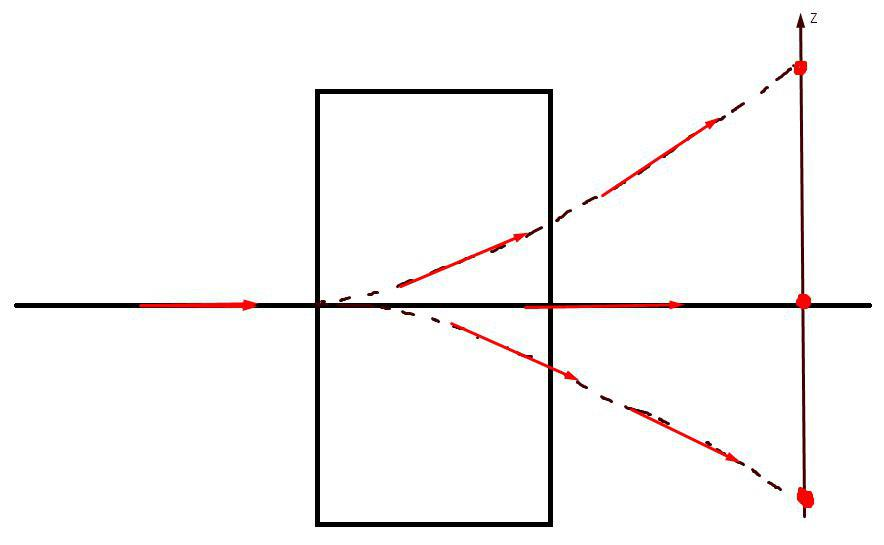
\includegraphics[width=0.9\linewidth]{ch-18.jpg}}
	\end{figure}
	\textbf{Гипотеза спина электрона}\\
	Подсчитаем число пучков на выходе из неоднородного $\vec{B}$. Вопрос: Сколько возможных $\mu_z$ ?
	\begin{gather*}
		\mu_z = -\mu_Bm
	\end{gather*}
	где $\mu_B$ - магнетон Бора.\\
	При фиксированном $l$ число возможных $m$ составляет $2l+1$ и учитывая, что $l,n \in N$, приходим к выводу, что число возможных $m$ - нечетное. Проверим это:\\
	Для этого пропустим пучок атомов водорода с $l=0$ через область неоднородного магнитного поля. Поскольку $l = 0 \Rightarrow m = 0 \Rightarrow \mu_z = 0 \Rightarrow$ пучок должен проследовать прямо в центр экрана, НО это не так - он расщепляется на две составляющие! Таким образом приходиться предположить, что электрон обладает собственным моментом импульса или спином, которому соответствует некоторый магнитный момент. Приходим к определению полного момента импульса частицы:
	\begin{gather*}
		\hat{J} = \hat{L}+\hat{S}
	\end{gather*} 
	где $\hat{L}$ - орбитальный момент, $\hat{S}$ - спин.\\\\
	Ввиду того (как оказалось), что электрон обладает внутренней степенью свободы(спином), то теперь для того, чтобы охарактеризовать его стационарные состояния в поле ядра нам потребуется уже не 3 квантовых числа а четыре (добавляется спиновое квантовое число - $m_s$)\\\\
	\textbf{Функция распределения Бозе-Эйнштейна}\\
	Функция распределения Бозе-Эйнштейна для частиц с целым (в том числе нулевым) спином имеет вид:
	$$f(\varepsilon) = 1/(e^{\frac{\varepsilon - \mu}{kT}} - 1)$$
	где $\varepsilon$ - кинетическая энергия частицы, $\mu$ - химический потенциал, зависящий от температуры.
	\textbf{Функция распределения Ферми-Дирака}\\
	Функция распределения Ферми-Дирака определяет вероятность заселения (из-за двух возможнх ориентаций спина на каждом уровне энергии могут находиться 2 электрона) уровня с энергией $\varepsilon$ и имеет вид:
	$$f(\varepsilon) = 1/(e^{\frac{\varepsilon - \varepsilon_F}{kT}} + 1)$$
	Здесь $\varepsilon_F$ - энергия Ферми, параметр, определяемый из очевидного условия, что сумма заселенности всех уровней энергии должна равняться полному числу электронов:
	$$\sum f(\varepsilon) = N_\varepsilon$$
	\textbf{Матрицы Паули}\\
	Если $s = \frac{1}{2}$, то возможны только два состояния
	\begin{gather}
	\left|\frac{1}{2}m_s\right>; \qquad m_s = \pm \frac{1}{2}
	\end{gather}
	Про состояние, котором проекция спина на направление $z$ положительна,говорят "спин вверх", запись же тоже сократим:
	\begin{gather}
	\left|\frac{1}{2}+\frac{1}{2}\right> \equiv \left|+\right>
	\end{gather}
	Когда проекция отрицательна "спин вниз":
	\begin{gather}
	\left|\frac{1}{2}-\frac{1}{2}\right> \equiv \left|-\right>
	\end{gather}
	Состояния $\left|+\right>$ и $\left|-\right>$\\
	- ортогональны (в силу того, что являются собственными векторами, отвечающими различным с.з. оператора $\hat{S}_z$): $\left<-|+\right> = \left<+|-\right> = 0$\\
	- норм. на единицу: $\left<-|=\right> = \left<+|+\right> = 1$\\
	Соотношения при $s=\frac{1}{2}$:
	\begin{gather}
	\hat{S}^2 \left|sm_s\right> = \hbar^2 s(s+1)\left|sm_s\right>\\
	\hat{S}_z \left|sm_s\right> = \hbar m_s \left|sm_s\right>\\
	\hat{S}_{\pm} \left|sm_s\right> = \hbar \sqrt{s(s+1)-m_s(m_s \pm 1)}\left|sm_s\pm 1\right>\\
	\hat{S}^2 \left|+\right> = \hbar \frac{3}{4} \left|+\right> \qquad \hat{S}_z\left|+\right>=\frac{\hbar}{2}\left|+\right> \qquad \hat{S}_+ \left|+\right> =0 \qquad \hat{S}_- \left|+\right> = \hbar \left|-\right>\\
	\hat{S}^2 \left|-\right> = \frac{3}{4}\hbar \left|-\right> \qquad \hat{S}_z \left|-\right> = -\frac{\hbar}{2}\left|-\right> \qquad \hat{S}_+ \left|-\right> = \hbar \left|+\right> \qquad \hat{S}_- \left|-\right> = 0\\
	\end{gather}
	Выпишим матрицы операторов $\hat{S}^2,\hat{S}_z,\hat{S}_{\pm}$ ($\hat{A}: A_{ij} \equiv \left<i|\hat{A}|j\right>$):
	\begin{gather}
	\hat{S}^2 = \left(\begin{matrix}
	\left<+|\hat{S}^2|+\right> & \left<+|\hat{S}^2|-\right> \\
	\left<-|\hat{S}^2|+\right> & \left<-|\hat{S}^2|-\right>
	\end{matrix}\right) = \frac{3}{4}\hbar^2
	\left(\begin{matrix}
	1 & 0\\
	0 & 1
	\end{matrix}\right)\\
	\hat{S}_z = \left(\begin{matrix}
	\left<+|\hat{S}_z|+\right> & \left<+|\hat{S}_z|-\right> \\
	\left<-|\hat{S}_z|+\right> & \left<-|\hat{S}_z|-\right>
	\end{matrix}\right) = \frac{\hbar}{2}
	\left(\begin{matrix}
	1 & 0\\
	0 & -1
	\end{matrix}\right)\\
	\hat{S}_+ = \left(\begin{matrix}
	\left<+|\hat{S}_+|+\right> & \left<+|\hat{S}_+|-\right> \\
	\left<-|\hat{S}_+|+\right> & \left<-|\hat{S}_+|-\right>
	\end{matrix}\right) = \hbar
	\left(\begin{matrix}
	0 & 1\\
	0 & 0
	\end{matrix}\right)\\
	\hat{S} = \left(\begin{matrix}
	\left<+|\hat{S}_-|+\right> & \left<+|\hat{S}_-|-\right> \\
	\left<-|\hat{S}_-|+\right> & \left<-|\hat{S}_-|-\right>
	\end{matrix}\right) = \hbar
	\left(\begin{matrix}
	0 & 0\\
	1 & 0
	\end{matrix}\right)\\
	\hat{S}_x = \frac{\hat{S}_+ + \hat{S}_-}{2} = \frac{\hbar}{2} \left(\begin{matrix}
	0 & 1\\
	1 & 0
	\end{matrix}\right)\\
	\hat{S}_y =\frac{\hat{S}_+ - \hat{S}_-}{2i} = \frac{\hbar}{2} \left(\begin{matrix}
	0 & -i\\
	i & 0
	\end{matrix}\right)\\
	\hat{\sigma}_z = \left(\begin{matrix}
	1 & 0\\
	0 & -1
	\end{matrix}\right)\\
	\hat{\sigma}_x = \left(\begin{matrix}
	0 & 1\\
	1 & 0
	\end{matrix}\right)\\
	\hat{\sigma}_y = \left(\begin{matrix}
	0 & -i\\
	i & 0
	\end{matrix}\right)\\
	\end{gather}
	Матрицы $(\hat{\sigma}_x),(\hat{\sigma}_y),(\hat{\sigma}_z)$ которые с точностью до множителя $\frac{\hbar}{2}$ совпадают $(\hat{S}_x),(\hat{S}_y),(\hat{S}_z)$	называются Матрицы Паули.\\	
\end{document}